% Manuscript prepared for Electronics (MDPI).
% This source is intended to be compiled inside the official MDPI LaTeX template.
% Replace placeholder author metadata before submission.
\documentclass[journal,article,submit,pdftex,moreauthors]{Definitions/mdpi}

%====================
% Metadata
%====================
\Title{Reconstructing LLM Outputs from SSE-Equivalent Application-Layer Length Traces: A Controlled Cross-Model and Defense Evaluation}

\Author{Author One $^{1,*}$ and Author Two $^{2}$}
\AuthorNames{Author One and Author Two}
\address[1]{Department/Institute, University/Organization, City, Country; author1@example.com}
\address[2]{Department/Institute, University/Organization, City, Country; author2@example.com}
\corres{Correspondence: author1@example.com}

\firstnote{Author identities, affiliations, funding, conflicts of interest, and the archival artifact DOI must be confirmed before submission.}

\pubvolume{1}
\issuenum{1}
\articlenumber{0}
\pubyear{2026}
\copyrightyear{2026}
\datereceived{}
\daterevised{}
\dateaccepted{}
\datepublished{}

%====================
% Packages
%====================
\usepackage{booktabs}
\usepackage{multirow}
\usepackage{graphicx}
\usepackage{array}
\usepackage{longtable}
\usepackage{tabularx}
\usepackage{threeparttable}
\usepackage{amsmath}
\usepackage{enumitem}
\usepackage{placeins}
\usepackage{tikz}
\usetikzlibrary{arrows.meta,positioning,shapes.geometric,fit}
\usepackage{pgfplots}
\pgfplotsset{compat=1.18}

%====================
% Abstract and keywords
%====================
\abstract{Large-language-model (LLM) assistants frequently stream responses token by token using Server-Sent Events (SSE). This paper evaluates reconstruction from instrumented, SSE-equivalent application-layer event lengths; it does not passively extract individual SSE frames from TLS, HTTP/2, or QUIC records. Across 2100 samples from seven open-weight models (300 aligned prompts per model), mean fixed-backend term-frequency cosine similarity $\phi$ ranged from 0.3242 for Qwen2.5-1.5B-Instruct (bootstrap 95\% CI $[0.3097,0.3380]$) to 0.0239 for Phi-3.5-mini-instruct ($[0.0201,0.0280]$). Paired Wilcoxon tests with Holm correction found 19 of 21 cross-model differences significant. We additionally evaluated five defensive configurations---8-byte bucketing, fixed 32-byte framing, two- and four-token batching, and randomized padding---against a frozen, non-adaptive reconstructor on two models. All ten defense--baseline comparisons remained significant after Holm correction, with observed leakage reductions of 35.0--90.3\%. No defended sample exceeded $\phi>0.5$, although the per-cell Wilson upper bound remained 11.35\%. These results quantify lexical leakage and mitigation potential under a controlled length oracle, but do not establish robustness against adaptive attackers or feasibility of an end-to-end passive network attack.}

\keyword{large language models; side-channel analysis; server-sent events; traffic analysis; privacy leakage; token streaming; text reconstruction; AI assistants}

\begin{document}

\section{Introduction}
Interactive LLM assistants commonly return answers incrementally to reduce perceived latency. A frequent implementation pattern is token streaming over Server-Sent Events (SSE), in which each emitted application-layer chunk is encapsulated in a text frame. Encryption protects payload content but not necessarily all traffic metadata. This study does not recover SSE frames passively from TLS records: it analyzes instrumented, SSE-equivalent application-layer traces in which one logged frame corresponds to one generated token.

The threat model follows the attack family introduced by Weiss \emph{et al.}, who showed that AI-assistant responses may leak through token-length side channels visible over the network~\cite{weiss2024prompt}. Our narrower experiment isolates the information contained in idealized application-layer length sequences. It does not model TLS record coalescing, HTTP/2 multiplexing, QUIC framing, fragmentation, proxy behavior, or the inference required to map encrypted records back to individual SSE events.

The study addresses three research questions:
\begin{enumerate}[label=\textbf{RQ\arabic*:},leftmargin=3.8em]
    \item How much lexical information can a fixed Weiss-style reconstructor recover from SSE-equivalent one-token-per-frame length traces across victim models?
    \item Are cross-model differences statistically distinguishable after prompt pairing and family-wise error correction?
    \item How effectively do bucketing, fixed framing, batching, and randomized padding reduce recovery, and at what byte/frame-count cost?
\end{enumerate}

The contribution of this paper is fourfold. First, we provide a controlled and artifact-audited methodology for collecting per-token application-layer traces. Second, we compare seven open-weight models using one fixed TF-cosine backend and aligned prompts. Third, we quantify uncertainty with bootstrap intervals, paired Wilcoxon tests, Holm correction, and rank-biserial effects. Fourth, we evaluate five defense configurations against a frozen non-adaptive reconstructor and report both residual leakage and overhead.

\section{Related Work}
Side-channel attacks infer sensitive information from indirect observables such as timing and message size. Classical timing attacks showed that implementation-level leakage can defeat cryptographic protection without recovering plaintext directly~\cite{kocher1996timing}. Network-encrypted applications likewise leak through packet sizes and timing: keystroke inference, web-application traffic analysis, and website fingerprinting demonstrate that encryption does not hide communication shape~\cite{song2001timing,chen2010sidechannel,cai2012touching,sirinam2018deep}.

Traffic-analysis defenses transform that shape through padding, morphing, batching, or cover traffic. Traffic morphing attempts to make one class resemble another, while subsequent studies show that efficient countermeasures often retain exploitable structure or impose substantial overhead~\cite{wright2009morphing,dyer2012peekaboo}. These trade-offs motivate reporting residual leakage together with bandwidth and latency costs rather than treating padding as a binary protection.

For generative AI, Weiss \emph{et al.} demonstrated remote reconstruction from token-length patterns and introduced T5-based sequence-to-text inversion~\cite{weiss2024prompt}. Later work examines merged LLM API outputs, where multiple tokens may share an observable unit~\cite{li2026length}, and Whisper Leak studies related encrypted-traffic inference against LLM interactions~\cite{whisperleak2025}. Relative to these studies, our contribution is not a new TLS extraction technique; it is a controlled cross-model benchmark of a fixed reconstructor, uncertainty-aware inference, and a defense pilot at the application-trace layer.

The reconstruction pipeline uses T5-style text-to-text transformers~\cite{raffel2020exploring}. Evaluation combines normalized Levenshtein distance~\cite{levenshtein1966binary}, ROUGE precision~\cite{lin2004rouge}, and a single fixed term-frequency cosine score $\phi$. Sentence-BERT~\cite{reimers2019sentence} is discussed as a future paraphrase-aware measure, but its scores are not mixed with the final publication results.

\section{Materials and Methods}
\subsection{Threat Model and Objective}
We evaluate an attacker that receives the ordered byte lengths of SSE-equivalent application-layer events generated by an instrumented LLM service. The attacker does not receive token text, prompts, or model internals. This is a length-oracle abstraction: unlike a fully passive network attacker, it does not need to infer application-event boundaries from TLS, HTTP/2, or QUIC traffic. Consequently, the results establish leakage conditional on obtaining token-granular lengths, not the feasibility of obtaining those lengths from an arbitrary production connection.

The primary objective is to determine how accurately assistant responses can be reconstructed from frame-length metadata alone. The experimental campaign therefore addressed three tasks: (i) capture per-token side-channel traces during live inference, (ii) reconstruct text from the resulting length sequences, and (iii) quantify reconstruction quality against ground-truth outputs.

\begin{figure*}[ht]
\centering
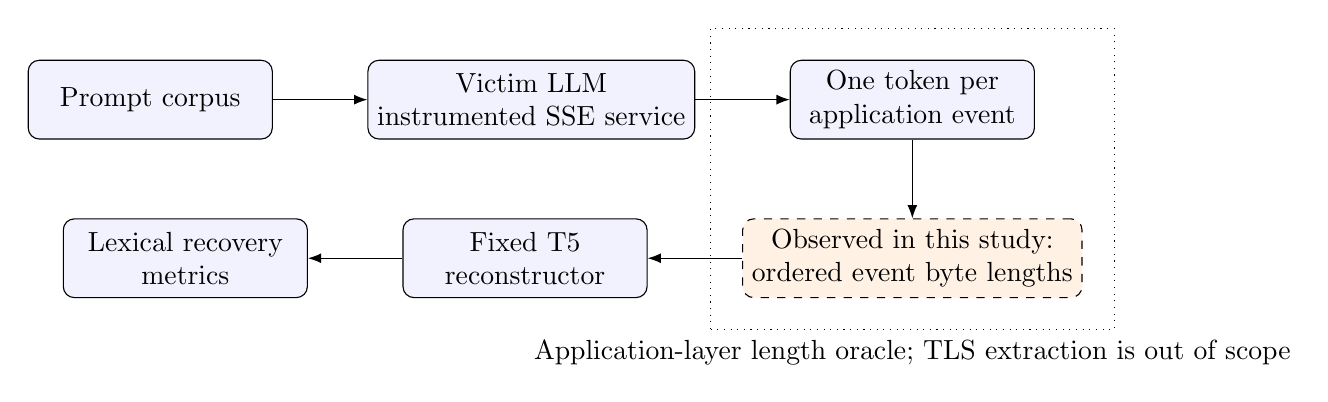
\begin{tikzpicture}[node distance=10mm and 12mm,>=Latex,
box/.style={draw,rounded corners,align=center,minimum height=10mm,minimum width=31mm,fill=blue!5},
obs/.style={draw,dashed,rounded corners,align=center,minimum height=10mm,minimum width=35mm,fill=orange!10}]
\node[box] (user) {Prompt corpus};
\node[box,right=of user] (victim) {Victim LLM\\instrumented SSE service};
\node[box,right=of victim] (stream) {One token per\\application event};
\node[obs,below=of stream] (oracle) {Observed in this study:\\ordered event byte lengths};
\node[box,left=of oracle] (attacker) {Fixed T5\\reconstructor};
\node[box,left=of attacker] (score) {Lexical recovery\\metrics};
\draw[->] (user)--(victim);
\draw[->] (victim)--(stream);
\draw[->] (stream)--(oracle);
\draw[->] (oracle)--(attacker);
\draw[->] (attacker)--(score);
\node[draw,dotted,fit=(stream)(oracle),inner sep=4mm,label=below:{Application-layer length oracle; TLS extraction is out of scope}] {};
\end{tikzpicture}
\caption{Threat model. The experiment begins at SSE-equivalent application-event lengths; it does not claim passive recovery of event boundaries from encrypted transport records.}
\label{fig:threat_model}
\end{figure*}

\subsection{Streaming Harness and Trace Collection}
The measurement harness implemented SSE streaming in a strict one-token-per-event configuration. Each application event followed the format \texttt{data: \textless token\textgreater\textbackslash n\textbackslash n}, while stream termination used \texttt{data: [DONE]\textbackslash n\textbackslash n}. For every emitted token, the harness logged token text for ground-truth evaluation, token UTF-8 length, application-event UTF-8 length, and relative emission timestamp. Per-run metadata additionally included the model identifier, decoding parameters, prompt, generated response text, and token count. The attacker-facing reconstruction input contained lengths only.

This design creates a direct mapping between tokens and transport-visible frames, which is essential for invertible side-channel analysis. Denoting the UTF-8 length of the $t$-th SSE frame by $L^{\mathrm{frame}}_t$, the estimated token length is
\begin{equation}
L^{\mathrm{tok}}_t = L^{\mathrm{frame}}_t - 8,
\end{equation}
where 8 bytes correspond to the fixed SSE overhead generated by the prefix \texttt{data: } and the suffix \texttt{\textbackslash n\textbackslash n}. The terminal \texttt{[DONE]} frame is excluded from reconstruction.

\subsection{Reconstruction Pipeline}
The inversion pipeline follows a Weiss-style sequence-to-text procedure. First, the token-length sequence is segmented heuristically into sentence-like chunks. Second, the initial chunk is decoded using \texttt{royweiss1/T5\_FirstSentences}. Third, subsequent chunks are decoded with \texttt{royweiss1/T5\_MiddleSentences} using preceding context. Finally, multiple decoding candidates are ranked according to aggregate generation confidence represented by the transition log-probability sum.

The reconstruction design is therefore conditional rather than purely tokenwise. Instead of recovering each token independently, it maps length patterns into coherent text spans and uses context to improve linguistic plausibility. Our quantitative claims nevertheless concern lexical recovery; semantic correctness was not established by human annotation.

\begin{figure*}[ht]
\centering
\begin{tikzpicture}[node distance=8mm,>=Latex,
step/.style={draw,rounded corners,align=center,minimum height=11mm,minimum width=27mm,fill=green!6}]
\node[step] (capture) {Event-length\\sequence};
\node[step,right=of capture] (norm) {Subtract fixed\\8-byte overhead};
\node[step,right=of norm] (segment) {Heuristic\\segmentation};
\node[step,right=of segment] (first) {First-sentence\\T5 decoding};
\node[step,right=of first] (middle) {Context-aware\\middle decoding};
\node[step,right=of middle] (rank) {Candidate ranking\\and concatenation};
\draw[->] (capture)--(norm);
\draw[->] (norm)--(segment);
\draw[->] (segment)--(first);
\draw[->] (first)--(middle);
\draw[->] (middle)--(rank);
\end{tikzpicture}
\caption{Reconstruction pipeline used for all victim models and defense transformations. The decoder checkpoints and ranking procedure remain fixed.}
\label{fig:pipeline}
\end{figure*}

\subsection{Prompt Corpus and Experimental Protocol}
The prompt corpus comprised 15 topical files with 20 prompts each, for a total of 300 prompts. Topics included legal issues, mental health, safety and security, sexual health, employment, financial status, and related sensitive categories. Prompt scheduling used round-robin interleaving across topics to reduce topical clustering effects.

Victim-model decoding was deterministic, with temperature set to 0.0 and \texttt{top\_p} set to 1.0. A typical run contained 300 prompts per model. For primary cross-model claims, a standardized subset was selected with the following shared parameters: $N=300$, \texttt{max\_new\_tokens}=96, \texttt{samples\_per\_segment}=3, \texttt{max\_sentences}=3, and \texttt{num\_first\_candidates}=3.

\subsection{Evaluation Metrics}
Reconstruction quality was computed using four complementary lexical criteria. The first was normalized Levenshtein distance (\texttt{ed\_norm}), which captures character-level divergence between the reconstruction and the reference. The second and third were ROUGE-1 precision and ROUGE-L precision, which quantify lexical overlap from unigram and longest-common-subsequence perspectives~\cite{lin2004rouge}. The final metric, $\phi$, was recomputed for every one of the 2100 samples as cosine similarity between term-frequency vectors of the reference and reconstruction.

In addition to mean metrics, the study reported a lexical recovery rate $\mathrm{LR}@0.5$, defined as the proportion of samples with $\phi > 0.5$. The threshold is a conventional operating point and has not been calibrated against human judgments. Importantly, the final publication analysis recomputed $\phi$ for all samples using one term-frequency cosine backend; it therefore measures lexical overlap rather than paraphrase-aware semantic equivalence.

\subsection{Statistical Analysis}
Because the same 300 prompts were issued to every model, cross-model inference used prompt-aligned observations. Mean metrics were accompanied by percentile bootstrap 95\% confidence intervals based on $B=10{,}000$ paired-index resamples with replacement and seed \texttt{20260706}. Confidence intervals for mean pairwise differences were obtained by bootstrapping the vector of within-prompt differences, thereby preserving pairing. Wilson 95\% intervals were used for $\mathrm{LR}@0.5$.

Pairwise differences in per-prompt $\phi$ were assessed using two-sided paired Wilcoxon signed-rank tests~\cite{wilcoxon1945individual}. Absolute nonzero differences received average ranks when tied; exact zero differences were removed (Wilcoxon convention). The implementation applies the standard tie correction to the normal-approximation variance and a continuity correction of 0.5. Therefore the effective $n$ is 300 for 18 pairs, 299 for two pairs, and 219 for TinyLlama versus Phi-3.5-mini. Holm--Bonferroni correction controlled family-wise error over all $\binom{7}{2}=21$ model pairs, and rank-biserial correlation quantified effect size~\cite{efron1994bootstrap,holm1979simple}. Defense--baseline comparisons used the same paired procedure with Holm correction over ten tests. Statistical significance was defined as adjusted $p<0.05$.

\subsection{Defense Evaluation Protocol}
Five configurations were evaluated on the same 30 topic-balanced prompts for each of Qwen2.5-1.5B-Instruct and Llama-3.2-3B-Instruct. Let $\ell_t$ denote the observable byte length of event $t$ before transformation.
\begin{itemize}[leftmargin=2em]
    \item \texttt{bucket\_8}: replace $\ell_t$ by $8\lceil \ell_t/8\rceil$, independently and online for every event.
    \item \texttt{pad\_32}: emit an online constant-width 32-byte protected payload unit; the evaluated implementation retains the application-event structure and accounts for bytes required to reach that unit.
    \item \texttt{batch\_2} and \texttt{batch\_4}: concatenate the lengths of consecutive groups of two or four tokens into one attacker-visible value. The final incomplete group, if present, is retained.
    \item \texttt{rand\_pad\_8}: add an independently sampled integer $U_t\sim\mathrm{Uniform}\{0,\ldots,8\}$ using a recorded deterministic seed.
\end{itemize}
The transformed length sequences were passed directly to the same segmentation and decoding pipeline. The reconstructor was frozen and was not retrained or calibrated on defended traces. Defense effectiveness was defined as $100(1-\bar\phi_d/\bar\phi_0)$. Byte overhead was computed from transformed versus original application payload-length sums; batching has zero overhead under this definition, which excludes record headers, buffering delay, and user-perceived latency. Mean observable frame count captures the structural cost of batching.

\subsection{Run Completeness Criteria}
A run was considered complete only if all required artifacts were present (\texttt{config.json}, \texttt{progress.json}, \texttt{samples.jsonl}, \texttt{summary.json}, \texttt{summary.md}, and \texttt{summary\_by\_topic.csv}) and if internal counts matched exactly, i.e.,
\begin{equation}
\texttt{progress.done} = \texttt{progress.total} = \texttt{summary.count} = \texttt{lines(samples.jsonl)}.
\end{equation}
These checks were applied before including any run in the main comparative analysis.

\section{Results}
\subsection{Completeness Audit}
The experiment directory contained 20 candidate execution folders, of which 14 were artifact-complete and 6 were incomplete placeholders. The complete runs contained 4050 samples in total. The prespecified standardized subset used for primary comparison covered seven models and 2100 samples. Each included model contributed exactly 300 samples. Execution identifiers are reported only in Appendix~\ref{app:runs}.

These results indicate that the core empirical dataset is sufficiently complete for model-level comparison under homogeneous settings. However, the presence of incomplete placeholders also underscores the importance of explicit artifact-completeness filters before aggregating results across runs.

\subsection{Cross-Model Comparison under Standardized Conditions}
Table~\ref{tab:main_results} reports the primary comparable subset using the fixed publication backend. Considerable variation is visible across victim models. Qwen2.5-1.5B-Instruct achieved the highest mean lexical similarity ($\phi=0.3242$), followed by Qwen2.5-3B-Instruct ($\phi=0.3096$), the base-model stress test Phi-1.5 ($\phi=0.2747$), and Llama-3.2-3B-Instruct ($\phi=0.2538$). Gemma-2-2B dropped to $\phi=0.1798$.

The lowest lexical reconstructability was observed for Phi-3.5-mini-instruct ($\phi=0.0239$) and TinyLlama-1.1B-Chat-v1.0 ($\phi=0.0428$). Phi-1.5 is not directly comparable as an instruction-following assistant; its relatively high fixed-backend score shows transfer of this reconstructor to base-model output style and must not be interpreted as evidence that base models are intrinsically more vulnerable. In terms of threshold recovery, only Qwen2.5-1.5B-Instruct exceeded an $8\%$ rate of samples with $\phi > 0.5$.

\begin{table*}[ht]
\centering
\caption{Primary cross-model comparison for the standardized subset using the fixed publication TF-cosine backend ($N=300$, \texttt{max\_new\_tokens}=96, \texttt{samples\_per\_segment}=3, \texttt{max\_sentences}=3, \texttt{num\_first\_candidates}=3).}
\label{tab:main_results}
\resizebox{\textwidth}{!}{%
\begin{tabular}{l l c c c c c}
\toprule
Model & Type & $\phi_{\mathrm{mean}}$ & $ed_{\mathrm{norm}}$ & R1 Precision & RL Precision & $\mathrm{LR}@0.5$ \\
\midrule
Qwen/Qwen2.5-1.5B-Instruct & instruct & 0.3242 & 0.7199 & 0.3220 & 0.2651 & 8.667\% \\
Qwen/Qwen2.5-3B-Instruct & instruct & 0.3096 & 0.7300 & 0.2945 & 0.2345 & 3.000\% \\
microsoft/phi-1\_5 & base & 0.2747 & 0.7426 & 0.2504 & 0.1891 & 4.333\% \\
meta-llama/Llama-3.2-3B-Instruct & instruct & 0.2538 & 0.7499 & 0.2387 & 0.1824 & 3.000\% \\
google/gemma-2-2b-it & instruct & 0.1798 & 0.7764 & 0.1719 & 0.1269 & 0.000\% \\
TinyLlama/TinyLlama-1.1B-Chat-v1.0 & chat & 0.0428 & 0.8026 & 0.0312 & 0.0310 & 0.000\% \\
microsoft/Phi-3.5-mini-instruct & instruct & 0.0239 & 0.8087 & 0.0158 & 0.0157 & 0.000\% \\
\bottomrule
\end{tabular}%
}
\end{table*}

\begin{figure*}[ht]
\centering
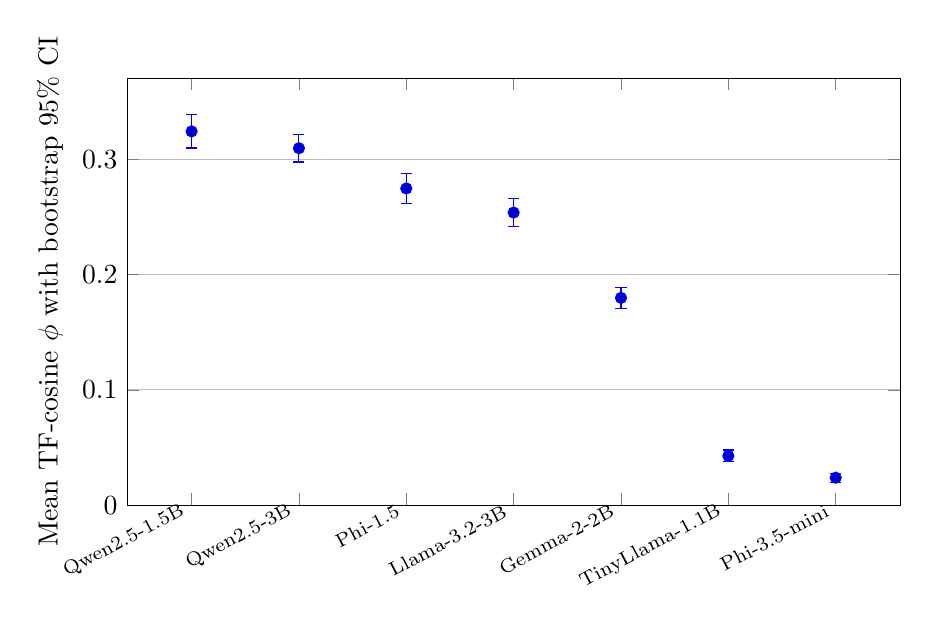
\begin{tikzpicture}
\begin{axis}[width=0.94\textwidth,height=7cm,ymin=0,ymax=0.37,
ylabel={Mean TF-cosine $\phi$ with bootstrap 95\% CI},
symbolic x coords={Qwen1.5,Qwen3,Phi1.5,Llama3,Gemma2,TinyLlama,Phi3.5},xtick=data,
xticklabels={Qwen2.5-1.5B,Qwen2.5-3B,Phi-1.5,Llama-3.2-3B,Gemma-2-2B,TinyLlama-1.1B,Phi-3.5-mini},
x tick label style={rotate=28,anchor=east,font=\scriptsize},ymajorgrids]
\addplot+[only marks,mark=*,blue,error bars/.cd,y dir=both,y explicit]
coordinates {(Qwen1.5,0.3242) +- (0,0.0144) (Qwen3,0.3096) +- (0,0.0119)
(Phi1.5,0.2747) +- (0,0.0128) (Llama3,0.2538) +- (0,0.0120)
(Gemma2,0.1798) +- (0,0.0091) (TinyLlama,0.0428) +- (0,0.0051)
(Phi3.5,0.0239) +- (0,0.0040)};
\end{axis}
\end{tikzpicture}
\caption{Mean lexical reconstruction score and bootstrap 95\% confidence intervals for the seven standardized runs. Error-bar half-widths are rounded to four decimals for visualization; the asymmetric endpoints are reported in Table~\ref{tab:statistical_results}.}
\label{fig:model_ci}
\end{figure*}

The historical per-run file for Phi-1.5 contains $\phi=0.0575$ and a 0.333\% threshold rate because it was generated with the backend available during that run. Those values are not used in this manuscript. All tables, confidence intervals, and hypothesis tests use the uniformly rescored per-prompt publication dataset, for which Phi-1.5 has mean $\phi=0.2747$ and $\mathrm{LR}@0.5=4.33\%$.

\subsection{Statistical Uncertainty and Pairwise Tests}
Table~\ref{tab:statistical_results} augments the point estimates with uncertainty intervals. Nineteen of 21 paired cross-model comparisons remained significant after Holm correction. The two exceptions were Qwen2.5-1.5B versus Qwen2.5-3B (mean paired difference 0.0146, 95\% CI $[-0.0026,0.0314]$, rank-biserial $r=0.089$, $p_{\mathrm{Holm}}=0.1838$) and Llama-3.2-3B versus Phi-1.5 (difference $-0.0209$, CI $[-0.0375,-0.0043]$, $r=-0.148$, $p_{\mathrm{Holm}}=0.0533$). In contrast, Qwen2.5-1.5B versus Phi-3.5-mini showed a large difference (0.3002, $r=1.000$, $p_{\mathrm{Holm}}<0.0001$). Thus, most observed gaps are distinguishable from prompt-sampling variation in this benchmark, but the tests do not establish causal model effects.

\begin{table*}[ht]
\centering
\caption{Uncertainty-aware results. Mean-$\phi$ intervals use 10,000 bootstrap resamples; $\mathrm{LR}@0.5$ intervals are Wilson 95\% intervals.}
\label{tab:statistical_results}
\begin{tabular}{l c c c c}
\toprule
Model & Mean $\phi$ & 95\% CI & $\mathrm{LR}@0.5$ & 95\% CI \\
\midrule
Qwen2.5-1.5B-Instruct & 0.3242 & [0.3097, 0.3380] & 8.67\% & [5.98, 12.40]\% \\
Qwen2.5-3B-Instruct & 0.3096 & [0.2977, 0.3214] & 3.00\% & [1.59, 5.60]\% \\
Phi-1.5 & 0.2747 & [0.2622, 0.2877] & 4.33\% & [2.55, 7.27]\% \\
Llama-3.2-3B-Instruct & 0.2538 & [0.2419, 0.2658] & 3.00\% & [1.59, 5.60]\% \\
Gemma-2-2B-it & 0.1798 & [0.1708, 0.1889] & 0.00\% & [0.00, 1.26]\% \\
TinyLlama-1.1B-Chat & 0.0428 & [0.0377, 0.0479] & 0.00\% & [0.00, 1.26]\% \\
Phi-3.5-mini-instruct & 0.0239 & [0.0201, 0.0280] & 0.00\% & [0.00, 1.26]\% \\
\bottomrule
\end{tabular}
\end{table*}

\subsection{Focused Comparison of Three Model Families}
Table~\ref{tab:new_models} isolates Llama-3.2-3B-Instruct, Gemma-2-2B-it, and Phi-3.5-mini-instruct as a focused cross-family comparison. Llama-3.2-3B-Instruct was the most reconstructable of the three, with $\phi=0.2538$ and a non-zero threshold recovery rate. Gemma-2-2B occupied a middle position with lower lexical scores. Phi-3.5-mini-instruct showed the strongest apparent resistance to this fixed pipeline, with near-zero lexical similarity and no samples above the $\phi > 0.5$ threshold.

This ordering holds under fully completed 300/300 runs and is therefore not an artifact of partial execution. Within the scope of the present pipeline, the relative ranking is Llama-3.2-3B $>$ Gemma-2-2B $>$ Phi-3.5-mini-instruct.

\begin{table}[ht]
\centering
\caption{Focused results for three victim-model families.}
\label{tab:new_models}
\resizebox{\columnwidth}{!}{%
\begin{tabular}{l c c c c c c}
\toprule
Model & Completion & $\phi_{\mathrm{mean}}$ & $ed_{\mathrm{norm}}$ & R1 & RL & $\mathrm{LR}@0.5$ \\
\midrule
Llama-3.2-3B-Instruct & 300/300 & 0.2538 & 0.7499 & 0.2387 & 0.1824 & 3.000\% \\
Phi-3.5-mini-instruct & 300/300 & 0.0239 & 0.8087 & 0.0158 & 0.0157 & 0.000\% \\
Gemma-2-2B & 300/300 & 0.1798 & 0.7764 & 0.1719 & 0.1269 & 0.000\% \\
\bottomrule
\end{tabular}%
}
\end{table}

\subsection{Exploratory Topic Sensitivity}
Selected topic-level summaries are shown in Table~\ref{tab:topic_sensitivity}. Although the available excerpt does not provide full per-topic distributions for all models, it indicates that topic sensitivity exists even within a fixed attack pipeline. For Llama-3.2-3B, the best topic was \emph{employment} ($\phi=0.3373$) and the worst was \emph{safety\_security} ($\phi=0.2053$). Gemma-2-2B performed best on \emph{beliefs\_values} and worst on \emph{financial\_status}. Phi-3.5-mini-instruct remained weak across both reported best and worst topics.

These descriptive observations suggest that leakage may depend on the linguistic distribution of generated content. The analysis is explicitly exploratory: it reports selected best/worst cells without multiplicity-corrected inference over all model--topic combinations and must not support confirmatory topic-level claims.

\begin{table}[ht]
\centering
\caption{Selected topic-level sensitivity based on mean fixed-backend lexical similarity.}
\label{tab:topic_sensitivity}
\begin{tabular}{l l c l c}
\toprule
Model & Best Topic & $\phi_{\mathrm{mean}}$ & Worst Topic & $\phi_{\mathrm{mean}}$ \\
\midrule
Llama-3.2-3B & employment & 0.3373 & safety\_security & 0.2053 \\
Gemma-2-2B & beliefs\_values & 0.2090 & financial\_status & 0.1575 \\
Phi-3.5-mini & financial\_status & 0.0444 & personal\_identity & 0.0073 \\
\bottomrule
\end{tabular}
\end{table}

\subsection{Effectiveness of Defensive Mechanisms}\label{sec:defense}
All ten paired defense--baseline comparisons remained significant after Holm correction ($p_{\mathrm{Holm}}\leq0.000589$). As shown in Table~\ref{tab:defense_results}, 8-byte bucketing provided the strongest consistently low residual leakage, reducing mean $\phi$ by 83.4--90.3\% with 82.4--88.6\% byte overhead. Two- and four-token batching reduced leakage by 67.7--69.2\% while reducing the observable frame count from 96 to 48 or 24 and introducing no payload-byte-sum overhead under the adopted accounting. Randomized padding reduced leakage by 61.0--65.7\%. The evaluated online fixed-32-byte implementation was least efficient, reducing leakage by only 35.0--36.8\% while adding 538--565\% byte overhead.

\begin{table*}[ht]
\centering
\caption{Defense effectiveness against the frozen non-adaptive reconstructor ($n=30$ paired prompts per model). Overhead excludes transport headers and latency.}
\label{tab:defense_results}
\begin{tabular}{l l c c c c c}
\toprule
Model & Defense & Mean $\phi$ & 95\% CI & Reduction & Byte overhead & Frames \\
\midrule
Qwen2.5-1.5B & baseline & 0.3010 & [0.2537, 0.3508] & -- & 0.0\% & 96 \\
 & bucket\_8 & 0.0293 & [0.0198, 0.0397] & 90.3\% & 82.4\% & 96 \\
 & pad\_32 & 0.1901 & [0.1667, 0.2150] & 36.8\% & 538.0\% & 96 \\
 & batch\_2 & 0.0928 & [0.0791, 0.1072] & 69.2\% & 0.0\% & 48 \\
 & batch\_4 & 0.0950 & [0.0668, 0.1269] & 68.4\% & 0.0\% & 24 \\
 & rand\_pad\_8 & 0.1033 & [0.0871, 0.1203] & 65.7\% & 78.5\% & 96 \\
\midrule
Llama-3.2-3B & baseline & 0.2576 & [0.2177, 0.2978] & -- & 0.0\% & 96 \\
 & bucket\_8 & 0.0428 & [0.0305, 0.0563] & 83.4\% & 88.6\% & 96 \\
 & pad\_32 & 0.1674 & [0.1382, 0.2003] & 35.0\% & 565.1\% & 96 \\
 & batch\_2 & 0.0823 & [0.0684, 0.0967] & 68.0\% & 0.0\% & 48 \\
 & batch\_4 & 0.0832 & [0.0615, 0.1055] & 67.7\% & 0.0\% & 24 \\
 & rand\_pad\_8 & 0.1004 & [0.0834, 0.1186] & 61.0\% & 81.9\% & 96 \\
\bottomrule
\end{tabular}
\end{table*}

\begin{figure}[ht]
\centering
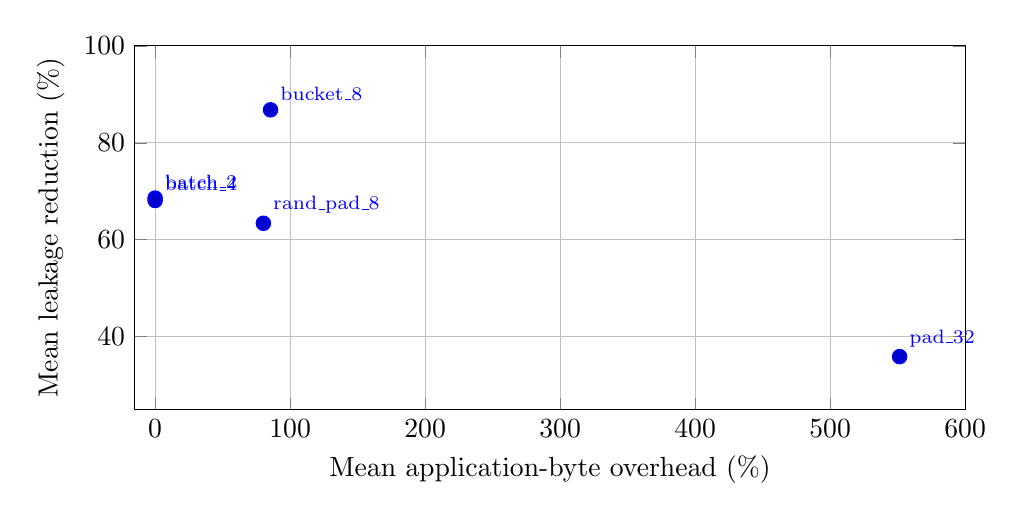
\begin{tikzpicture}
\begin{axis}[width=\columnwidth,height=6.2cm,xmin=-15,xmax=600,ymin=25,ymax=100,
xlabel={Mean application-byte overhead (\%)},ylabel={Mean leakage reduction (\%)},grid=major,
nodes near coords,point meta=explicit symbolic,every node near coord/.append style={font=\scriptsize,anchor=south west}]
\addplot+[only marks,mark=*,mark size=2.6pt,blue]
coordinates {(85.5,86.8) [bucket\_8] (551.5,35.9) [pad\_32]
(0,68.6) [batch\_2] (0,68.1) [batch\_4] (80.2,63.4) [rand\_pad\_8]};
\end{axis}
\end{tikzpicture}
\caption{Defense effectiveness versus mean application-byte overhead, averaged over the two evaluated models. Batching overlaps at zero byte-sum overhead but changes frame count and latency, which are not represented on the horizontal axis.}
\label{fig:defense_tradeoff}
\end{figure}

No defended sample exceeded $\phi>0.5$. With only 30 samples per defense/model cell, however, the Wilson 95\% upper bound is 11.35\%; zero observed recoveries must therefore not be interpreted as zero residual risk. These results demonstrate mitigation against the evaluated frozen attacker, not robustness against an adaptive reconstructor trained on defended traces.

\section{Discussion}
\subsection{Interpretation of Leakage Differences}
The results show that output leakage through SSE frame-length metadata is not uniform across models. Under identical collection and reconstruction settings, some models exhibited higher reconstruction scores than others within the evaluated benchmark. This finding matters operationally because a service that appears protected at the transport layer may still expose model-dependent potential privacy implications through streaming granularity and tokenization behavior.

At the same time, the present study does not claim a mechanistic explanation for why a given model is more or less reconstructable. The observed variation may reflect interactions among tokenizer behavior, output style, response length distributions, and the compatibility of generated traces with the reconstruction models. Isolating these factors requires dedicated ablation experiments and should therefore be treated as future work rather than as a conclusion of the present dataset.

\subsection{Practical Exploitability}
The threshold results indicate that high-quality semantic recovery is not universal, but the observed attack success rates indicate the potential for practical exploitation in some configurations, although additional evaluation is needed under production conditions. Even moderate mean similarity can be problematic when the attacked content concerns sensitive domains such as employment, legal issues, or mental health. Moreover, an adversary may combine multiple weak signals, repeated queries, or confidence-based re-ranking to improve practical recovery beyond what single-pass averages suggest.

A second practical lesson is methodological: attack efficacy metrics, exploitability metrics, and defense metrics should be reported separately. Mean lexical similarity captures aggregate word overlap, but does not by itself establish semantic correctness or actionability. Future studies should combine lexical scores, a fixed paraphrase-aware metric, and blinded human judgments.

\subsection{Limitations}
This study has several limitations. First, the primary comparison is intentionally restricted to a homogeneous subset; runs outside this subset should not be pooled for strong model-level claims. Second, $\phi$ is a lexical-overlap metric and does not establish semantic correctness. Stored artifacts contain reference and reconstructed texts, but no blinded human ratings or uniformly computed paraphrase-aware scores; neither is retroactively claimed in this paper. Third, deterministic victim decoding improves control but does not represent all deployed settings. Fourth, the defense pilot covers only two models and 30 prompts per cell, and the attacker was not retrained on defended traces. Fifth, multi-seed reconstruction variability, end-to-end encrypted-record extraction, latency, protocol-header overhead, and user-experience costs remain unmeasured.

For these reasons, the reported numbers should be interpreted as a carefully controlled baseline rather than a complete characterization of streaming-side-channel risk.

\subsection{Ethical Considerations}
This work is positioned as defensive security research. The goal is to quantify leakage risk in order to motivate safer streaming implementations and more realistic privacy assessments for AI assistants. Because the attack targets potentially sensitive outputs, public release of artifacts should be handled responsibly, with careful consideration of redaction, disclosure timing, and the inclusion of mitigations.

\section{Conclusions}
This paper presented an experimental evaluation of response reconstruction from SSE-equivalent application-layer length traces in token-streaming LLM assistants. Using an artifact-validated dataset and a Weiss-style reconstruction pipeline, we showed that lexical leakage remains measurable across multiple open-weight models and that transfer of the fixed reconstructor differs substantially across victim outputs.

Within the standardized comparison subset, the Qwen2.5 variants achieved the highest mean reconstruction metrics, whereas Phi-3.5-mini-instruct achieved the lowest. In the focused three-family comparison, the observed ordering was Llama-3.2-3B $>$ Gemma-2-2B $>$ Phi-3.5-mini-instruct. These results are conditional on an ideal application-layer length oracle; further research is needed to evaluate encrypted-record extraction, alternative deployment configurations, adaptive reconstruction, and production defense costs.

The most important next steps are to add a fixed paraphrase-aware semantic metric and blinded human evaluation, model stochastic reconstruction explicitly, retrain adaptive attackers on each defended trace distribution, and measure latency and bandwidth costs at the transport layer. Such extensions are necessary before making stronger claims about deployment-grade exploitability or mitigation efficacy.

Importantly, the present study evaluates leakage under a controlled laboratory setting and should not be interpreted as a direct assessment of any specific commercial AI service. Further work is required to determine the extent to which the observed effects generalize to real-world deployments.

\appendixtitles{yes}
\appendixstart

\appendix
\section{Artifact-Completeness Rules and Execution Identifiers}\label{app:runs}
For reproducibility, a run should be included in comparative analyses only if all required files are present and all internal sample counts match exactly. In the present campaign, the required files were \texttt{config.json}, \texttt{progress.json}, \texttt{samples.jsonl}, \texttt{summary.json}, \texttt{summary.md}, and \texttt{summary\_by\_topic.csv}. Any placeholder or partially completed run directory should be excluded from primary cross-model claims.

\begin{table}[ht]
\centering
\caption{Execution identifiers for the standardized publication subset.}
\begin{tabular}{l l}
\toprule
Model & Execution identifier \\
\midrule
Qwen2.5-1.5B-Instruct & \texttt{run\_20260325\_104518\_qwen\_1\_5b} \\
Qwen2.5-3B-Instruct & \texttt{run\_20260327\_124817\_qwen\_3b\_final\_resume} \\
Phi-1.5 & \texttt{run\_20260329\_085714\_phi\_1\_5} \\
Llama-3.2-3B-Instruct & \texttt{run\_20260414\_073030\_llama\_3\_2\_3b} \\
Gemma-2-2B-it & \texttt{run\_20260415\_080034\_gemma\_2\_2b\_it} \\
TinyLlama-1.1B-Chat & \texttt{run\_20260325\_153010\_tinyllama\_1\_1b} \\
Phi-3.5-mini-instruct & \texttt{run\_20260414\_111644\_phi\_3\_5\_mini} \\
\bottomrule
\end{tabular}
\end{table}

\authorcontributions{Conceptualization, Author One and Author Two; methodology, Author One; software, Author One; validation, Author One; formal analysis, Author One and Author Two; investigation, Author One; data curation, Author One; writing---original draft preparation, Author One; writing---review and editing, Author One and Author Two; supervision, Author Two. All authors have read and agreed to the published version of the manuscript. Author names and roles must be confirmed before submission.}
\funding{Funding information must be confirmed by the authors before submission.}
\institutionalreviewboardstatement{Not applicable. This study evaluated software systems and generated model outputs and did not involve human participants or identifiable personal data.}
\informedconsentstatement{Not applicable.}
\dataavailabilitystatement{The per-sample measurements, aligned publication metrics, statistical outputs, defense results, analysis scripts, and reproducibility manifest are included in the accompanying artifact package under \texttt{experiment\_validation/}. A persistent public repository URL and archival DOI must be inserted before submission.}
\conflictsofinterest{The authors must provide and confirm the conflict-of-interest statement before submission.}

\reftitle{References}
\bibliography{references}

\end{document}
